\documentclass{article}

\usepackage{algorithm}
%\usepackage{algorithmic}
\usepackage{algpseudocode}
\usepackage{bm}
\usepackage{amsmath}
\usepackage{amssymb}
\usepackage{amsfonts}
\usepackage{amsthm}
\usepackage{mathrsfs}
\usepackage[obeyspaces]{url}
\usepackage[colorlinks,linkcolor=blue]{hyperref}
%\usepackage{biblatex}

\theoremstyle{plain} \newtheorem{thm}{Theorem}

\usepackage{epsfig}
\renewcommand{\algorithmicrequire}{\textbf{Input:}} % Use Input in the format of Algorithm
\renewcommand{\algorithmicensure}{\textbf{Output:}} % Use Output in the format of Algorithm
\newcommand{\cA}{\mathcal{A}}
\newcommand{\cL}{\mathcal{L}}
\newcommand{\cF}{\mathcal{F}}
\usepackage{multirow}
\usepackage{subfigure}
\usepackage{graphicx}
\usepackage{float}
\usepackage{booktabs}
\usepackage{listings}
\usepackage{xcolor}
\definecolor{mygreen}{rgb}{0,0.6,0}
\definecolor{mygray}{rgb}{0.5,0.5,0.5}
\definecolor{mymauve}{rgb}{0.58,0,0.82}
\lstset{
	backgroundcolor=\color{white}, 
	basicstyle = \footnotesize,       
	breakatwhitespace = false,        
	breaklines = true,                 
	captionpos = b,                    
	commentstyle = \color{mygreen}\bfseries,
	extendedchars = false,             
	frame =shadowbox, 
	framerule=0.5pt,
	keepspaces=true,
	keywordstyle=\color{blue}\bfseries, % keyword style
	language = MATLAB,                     	% the language of code
	otherkeywords={string}, 
	numbers=left, 
	numbersep=10pt,
	numberstyle=\tiny\color{mygray},
	rulecolor=\color{black},         
	showspaces=false,  
	showstringspaces=false, 
	showtabs=false,    
	stepnumber=1,         
	stringstyle=\color{mymauve},        % string literal style
	tabsize=2,          
	title=\lstname                      
}

\setlength\parskip{.3\baselineskip}


\title{Report for Homework 1}
\author{Runyu Zhang}

\begin{document}
	\maketitle
\section{Problem Description}
Use the total variation model to deblur and denoise images.
\begin{equation*}
	\hat{u} = \mathop{\arg\min}_u \lambda \int |\nabla u| dx + \frac{1}{2} \int (\cA u - f)^2dx
\end{equation*}
where $f$ is the image to be deblurred and denoised. $\cA$ is the convolution operator with kernel $k$:
$$\cA u = k * u.$$
Here we choose the kernel to be gaussian. In implementation $k$ is generated by the matlab command \text{k = fspecial('gaussian', [s,s], sigma)}. Here s and sigma are predetermined parameters for the model.

\section{Scheme Design}
\subsection{Formulation of the Optimization Algorithm}
We use ADMM to solve this optimization problem:
$$\min_u \lambda||W u||_1 +\frac{1}{2}||A u - f||_2^2,$$
where $A$ and $W$ are the discretized convolution and gradient operator respectively.

The problem can be reformulated as:
\begin{align*}
&\min_{u, d} \lambda||d||_1 +\frac{1}{2}||A u - f||_2^2\\
&\text{s.t}\quad d = Wu.
\end{align*}

Write out the augment Lagrangian as follow:
$$\cL(u, d, p) = \lambda||d||_1 +\frac{1}{2}||A u - f||_2^2 +  <p, Wu - d> + \frac{\mu}{2} ||Wu - d||_2^2$$

Then the ADMM scheme can be derived by solving the following problem using coordinate descent:
$$\min_{u, d} \max_{p} \cL(u, d, p).$$

i.e.:
\begin{align*}
	d_k &= \mathop{\arg \min}_d \cL(u_{k-1}, d, p_{k-1})\\
		   &= \text{shrink}(Wu_{k-1} + \frac{1}{\mu}p_{k-1}, \frac{\lambda}{\mu})\\
	u_k &= \mathop{\arg \min}_u \cL(u, d_{k-1}, p_{k-1})\\
		   &= (A^TA + \mu W^TW)^{-1} (A^T f + \mu W^T d - W^T p)\\
	p_k &= p_{k-1} + \mu (Wu - d)
\end{align*}

\subsection{Boundary Condition for the Convolution Operator}
The updating of $u_k$ is the step that takes the most computational time, since it requires solving a linear equation system. However, if the boundary condition for both the convolution operator and the gradient operate is periodic, then this step can be accelerated via Fast Fourier Transform.

The updating of $u_k$ can be written as:
\begin{align*}
		u_k &= \mathop{\arg \min}_u \cL(u, d_{k-1}, p_{k-1})\\
				&= \mathop{\arg \min}_u   \lambda||d||_1 +\frac{1}{2}||A u - f||_2^2 +  <p, Wu - d> + \frac{\mu}{2} ||Wu - d||_2^2\\
				&= \mathop{\arg \min}_u \frac{1}{2}||A u - f||_2^2 + <p, Wu> + \frac{\mu}{2} ||Wu - d||_2^2\\
				& =  \mathop{\arg \min}_u \frac{1}{2}||A u - f||_2^2  + \frac{\mu}{2} ||Wu - (d - \frac{1}{\mu} p)||_2^2\\
\end{align*}
According to Parseval Equation, we have
\begin{align*}
	u_k &= \mathop{\arg \min}_u \frac{1}{2}||\cF(A)\cdot\cF(u) - \cF(f)||_2^2 + \frac{\mu}{2} ||\cF(W)\cdot\cF(u) - \cF(d - \frac{1}{\mu} p)||_2^2\\
	& =\cF^{-1}\left( \frac{\overline{\cF(A)}\cF(f) + \mu \overline{\cF(W)} \cF(d - \frac{1}{\mu} p)}{\overline{\cF(A)}\cF(A) + \mu \overline{\cF(W)} \cF(W)}\right)
\end{align*}
Here, $\cF$ denotes Fourier Transform,  the multiplication and devision are element-wise multiplication and devision. 

\subsection{Derivation of the Transpose Operator}
If the boundary condition for the convolution operator is not periodic, then we need to solve the linear equation system:
$$ (A^TA + \mu W^TW) u = A^T f + \mu W^T(d - \frac{1}{\mu}p)$$
Here we use conjugate gradient to solve the following equation. Since the gradient operator can also be viewed as a special convolution operator, we only need to find the operator that corresponds to the transpose of convolution. For simplicity, we consider 1-d convolution here, but the derivation of 2-d convolution is almost identical.

By the definition of transpose, we have:
\begin{align*}
	<A^Ty, x> &= <y, Ax> = <y, k*x>\\
	& = \sum_{i=0}^{n}y_i(\sum_{j=0}^{i}k_{i-j} x_{j})\\
	& = \sum_{j=0}^{n} x_{j} \sum_{i=j}^{n} k_{i-j}y_i\\
\end{align*} 
Thus we know that:
$$(A^Ty)_j = \sum_{i=j}^n k_{i-j}y_i $$
Thus we have:
$$(A^Ty)_{n-j} = \sum_{i=n-j}^n k_{i-n + j}y_i $$
By doing the index substitution: $i' = n - i$, we have:
$$(A^Ty)_{n-j} = \sum_{i'=0}^{j} k_{j-i'}y_{n-i'}$$
Thus, if we define a new vector $y'$ so that: $y'_{i} = y_{n-i}$, we will have:
$$(A^Ty)_{n-j} = \sum_{i=0}^{j} k_{j-i}y'_{i}$$
Thus the transpose operator can be calculated as:
\begin{algorithm}
	\begin{algorithmic}[1]
		\caption{Transpose Operator}
		\Require The convolution kernel $k$, the vector $y$
		\Ensure The vector $A^Ty$, which is the transpose of the convolution acting on the vector $y$
		\State Reverse the vector $y$: $y = y(end:-1:1)$;
		\State convolve the vector $y$ with $k$: $y = k*y$;
		\State Reverse the vector again: $y = y(end:-1:1)$;
		\State Output $y$.
	\end{algorithmic}
\end{algorithm}
\subsection{Duality of the Optimization Problem}
Since we use ADMM to solve the optimization problem, it might be helpful to write out the duality of the primal problem. The duality gap can also be used as a stopping criterion for the algorithm.

The primal problem is:
\begin{align*}
&\min_{u, d} \lambda||d||_1 +\frac{1}{2}||A u - f||_2^2\\
&\text{s.t}\quad d = Wu.
\end{align*}

The Lagrangian of this problem is:
\begin{align*}
	L(u, d, p) & = \frac{1}{2}||Au - f||_2^2 + \lambda ||d||_1 + <p, Wu - d>\\
		& = (\lambda ||d||_1 - <p, d>) + (\frac{1}{2}||Au - f||_2^2 + <p, Wu>) 
\end{align*}

The dual problem is $\inf_{u,d} =  (\lambda ||d||_1 - <p, d>) + (\frac{1}{2}||Au - b||_2^2 + <p, Wu>) $. In order for the first term $\inf_{d} \lambda ||d||_1 - <p, d>$ not to be $-\infty$, we must and the constraint :$$\lambda \mathbf{1} \ge p \ge -\lambda \mathbf{1}.$$

For the second term: $\inf_u = \frac{1}{2}||Au - f||_2^2 + <p, Wu>$, we have:
$$u = (A^TA)^{-1}(A^Tf - W^T p)$$

Thus we have: $$\inf_u = -\frac{1}{2}(A^Tf - W^Tp)^T()^{-1}(A^Tf - W^Tp) + \frac{1}{2} f^Tf.$$

Then the dual problem is
\begin{align*}
	\max_{p} & -\frac{1}{2}(A^Tf - W^Tp)^T()^{-1}(A^Tf - W^Tp) + \frac{1}{2} f^Tf\\
	&\qquad	\text{s.t.} \quad \lambda \mathbf{1} \ge p \ge -\lambda \mathbf{1}.
\end{align*}

The duality gap can be used as a stopping criterion, but strangely, for this problem, \textbf{the duality gap does not seem to converge to zero for $\lambda \le 10!$} But still, the deblurring and denoising results are acceptable. I still haven't figured out what is the problem up till now.
\section{Numerical Results}
For more detailed experimental results, see Appendix and 'results.pdf'
\subsection{Periodic Boundary Condition}
% Table generated by Excel2LaTeX from sheet 'Sheet1'
\begin{table}[htbp]
	\centering
	\caption{Experimental Results for Periodic Boundary Condition}
	\begin{tabular}{c|cccc}
		\toprule[.07cm]
		Image & Kamiya & Shizuwo & Classic & Koala \\
		\midrule[.07cm]
		recovered PSNR & 28.3532 & 25.4685 & 24.3043 & 29.8847 \\
		blurred PSNR & 23.4197 & 22.8125 & 23.2668 & 27.9442 \\
		\midrule
		recovered SSIM & 0.9315 & 0.9258 & 0.9227 & 0.9127 \\
		blurred SSIM & 0.8434 & 0.853 & 0.9046 & 0.8725 \\
		\bottomrule[.07cm]
	\end{tabular}%
	\label{tab:1}%
\end{table}%

For an image of size 716*500*3, the running time is 14.5 s
\subsection{Non-Periodic Boundary Condition}
% Table generated by Excel2LaTeX from sheet 'Sheet1'
\begin{table}[htbp]
	\centering
	\caption{Experimental Results for Non-Periodic Boundary Condition}
	\begin{tabular}{c|cccc}
		\toprule[.07cm]
		Image & Kamiya & Shizuwo & Classic & Koala \\
		\midrule[.07cm]
		recovered PSNR & 28.0124 & 25.4396 & 24.293 & 29.957 \\
		blurred PSNR & 22.5695 & 22.2524 & 22.7652 & 27.6617 \\
		\midrule
		recovered SSIM & 0.9128 & 0.9132 & 0.9222 & 0.9132 \\
		blurred SSIM & 0.8193 & 0.8355 & 0.8979 & 0.8708 \\
		\bottomrule[.07cm]
	\end{tabular}%
	\label{tab:2}%
\end{table}%

For an image of size 716*500*3, the running time is 139 s
\subsection{Some Observation}
\begin{itemize}
	\item The larger $\lambda$ is, the more robust to noise is the algorithm.
	\item Smaller $\lambda$ seems to lead to better deblurring results, but may have ringing effects caused by noise.
	\item The choice of $\mu$ cannot be too large, or the recovered image will still be blurred. (See 'results.pdf')
	\item We don't need to wait until the algorithm converges to the optimal points. Results gotten by twenty iterations does not seem to have much difference between results gotten by a hundred iterations.
\end{itemize}

\section{Appendix}
\begin{figure}
	\caption{\textbf{Experimental Results for Periodic Boundary Condition:} The picture on the left is the blurred image, on the right the recovered}
	\begin{minipage}{.5\linewidth}
		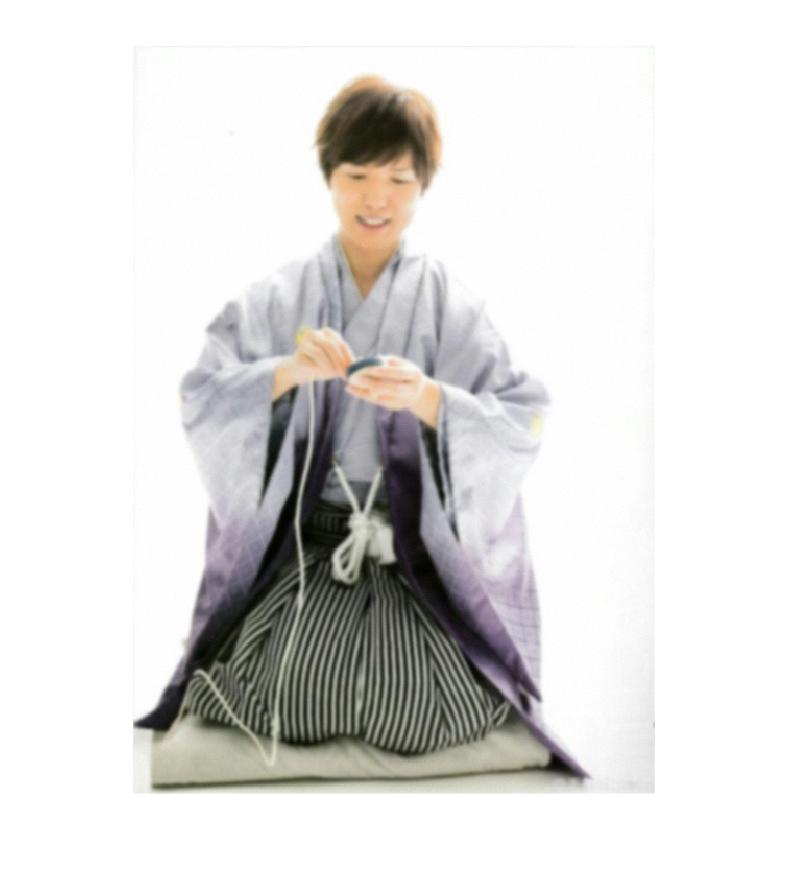
\includegraphics[width=\textwidth]{kamiya_blurred_cyclic.jpg}
	\end{minipage}
	\begin{minipage}{.5\linewidth}
		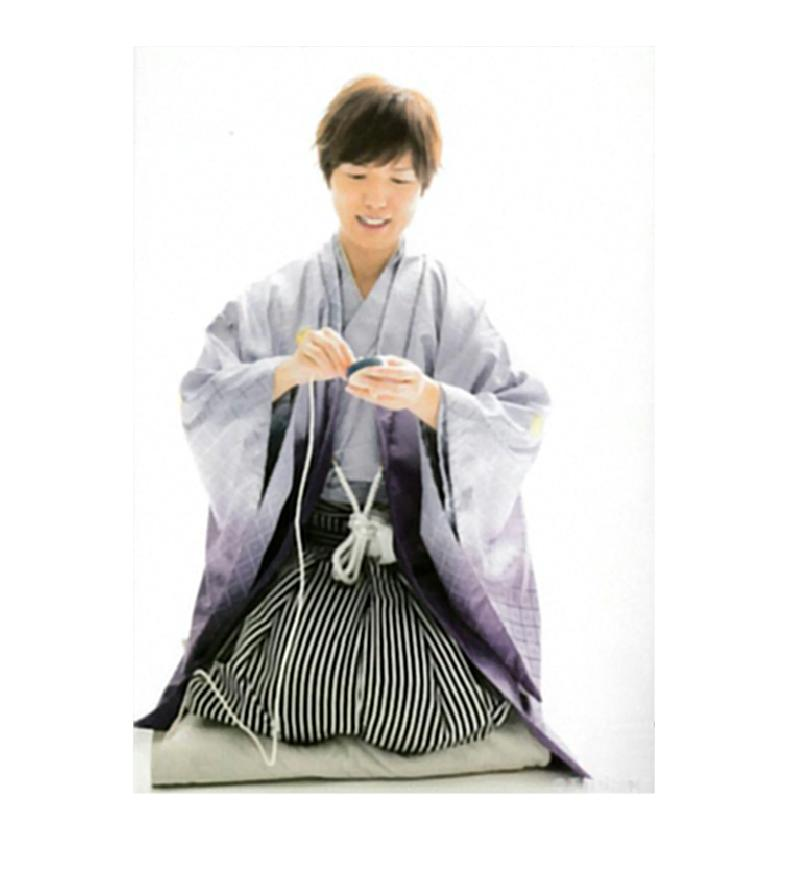
\includegraphics[width=\linewidth]{kamiya_recovered_cyclic.jpg}
	\end{minipage}
	\begin{minipage}{.5\linewidth}
		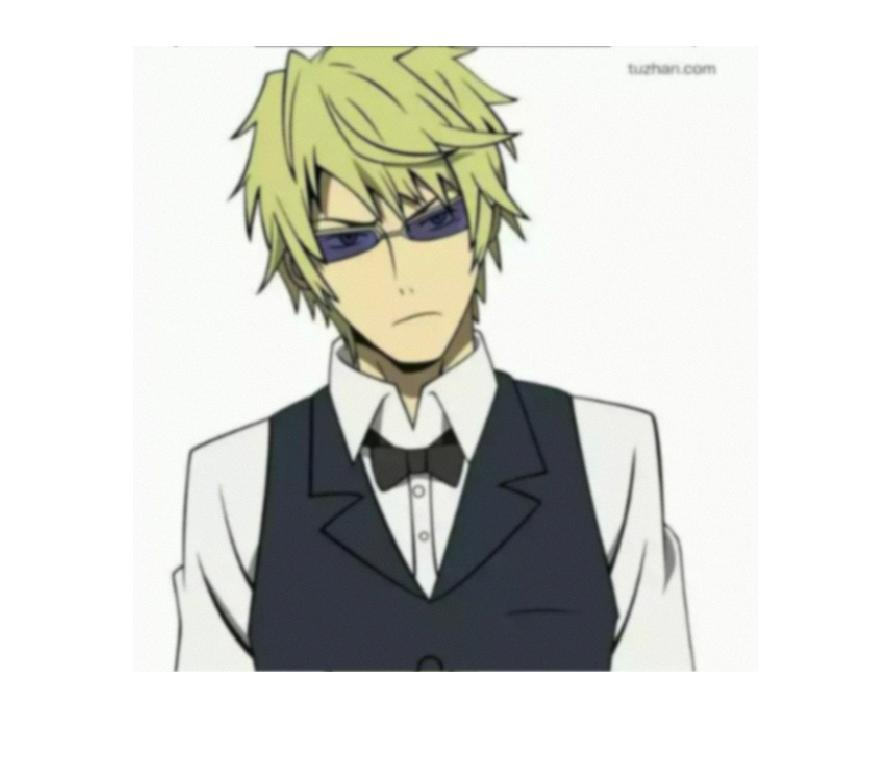
\includegraphics[width=\textwidth]{shizuwo_blurred_cyclic.jpg}
	\end{minipage}
	\begin{minipage}{.5\linewidth}
		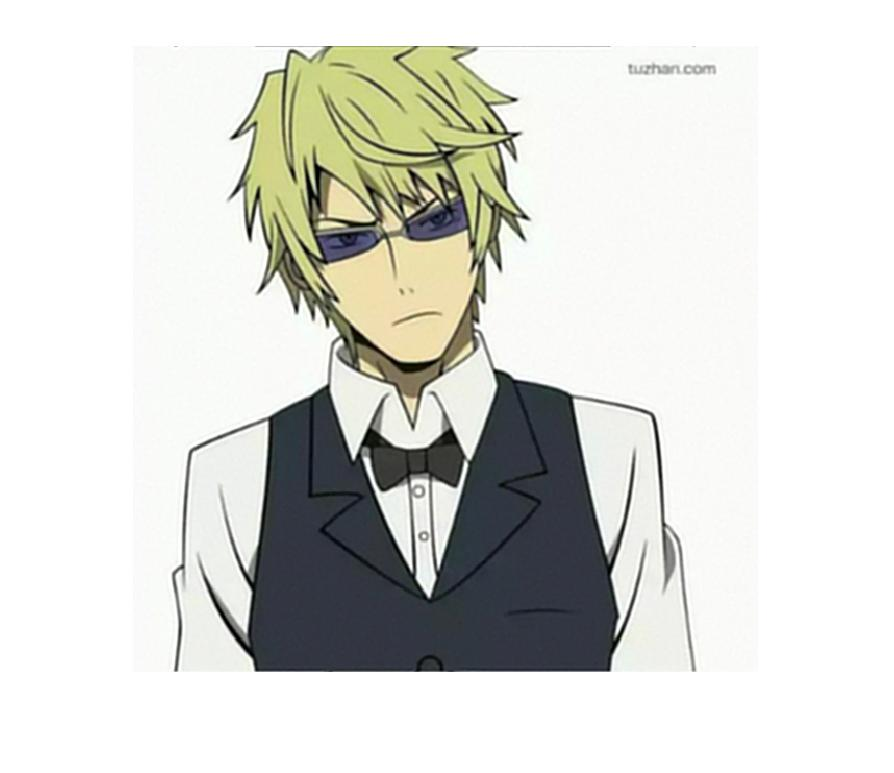
\includegraphics[width=\linewidth]{shizuwo_recovered_cyclic.jpg}
	\end{minipage}
	\begin{minipage}{.5\linewidth}
		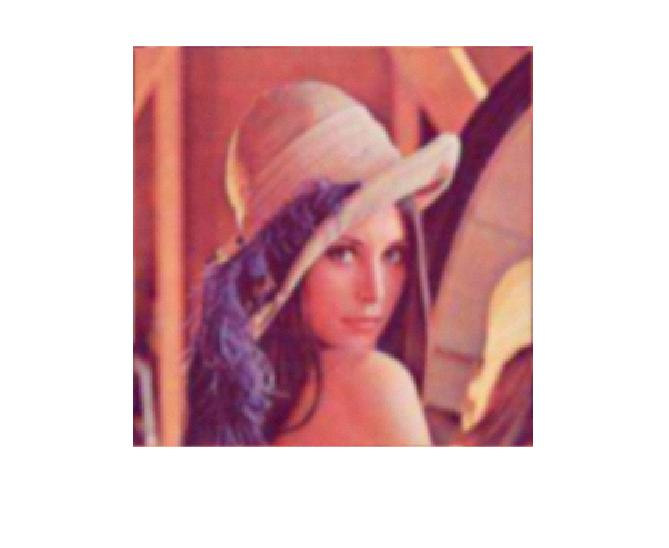
\includegraphics[width=\textwidth]{classic_blurred_cyclic.jpg}
	\end{minipage}
	\begin{minipage}{.5\linewidth}
		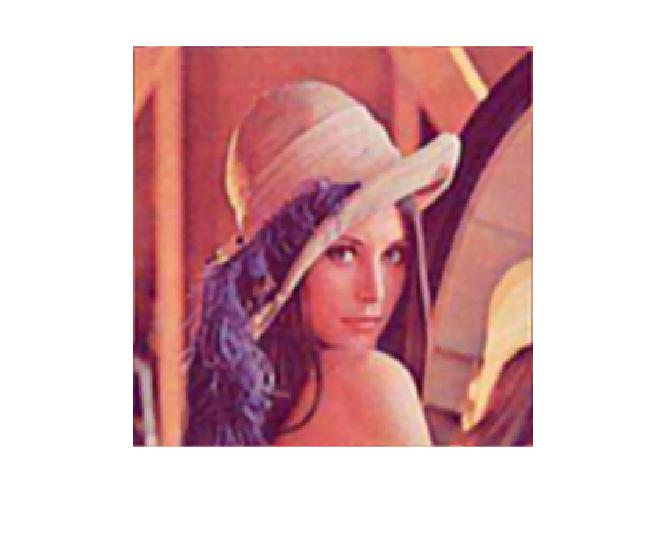
\includegraphics[width=\linewidth]{classic_recovered_cyclic.jpg}
	\end{minipage}
	\begin{minipage}{.5\linewidth}
		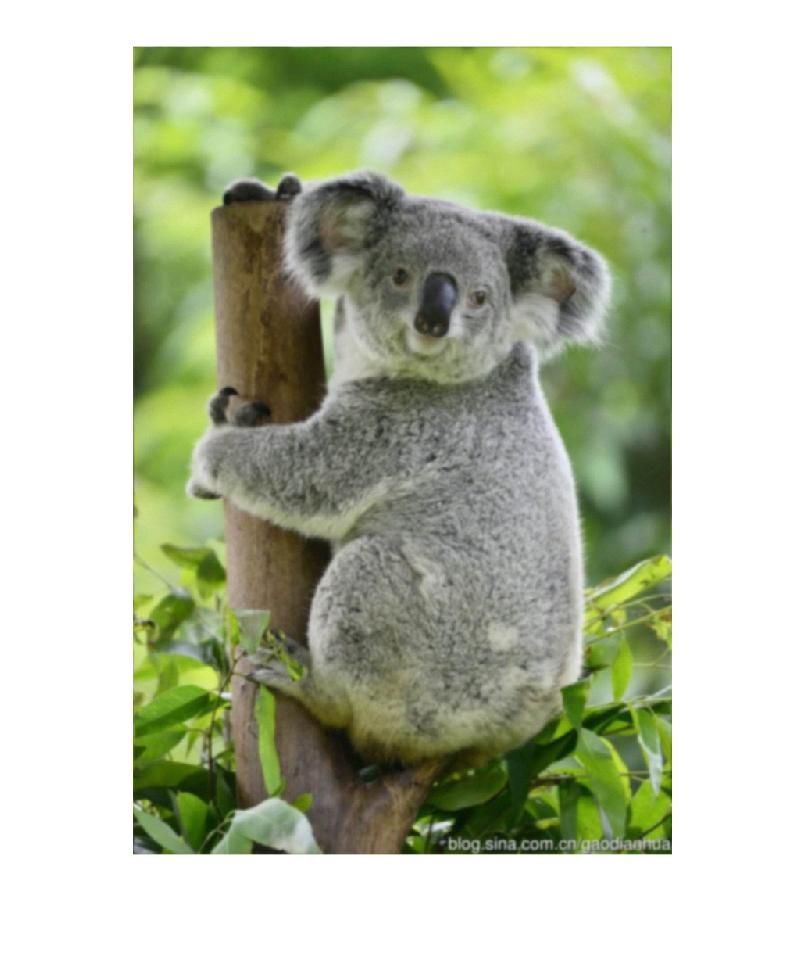
\includegraphics[width=\textwidth]{koala_blurred_cyclic.jpg}
	\end{minipage}
	\begin{minipage}{.5\linewidth}
		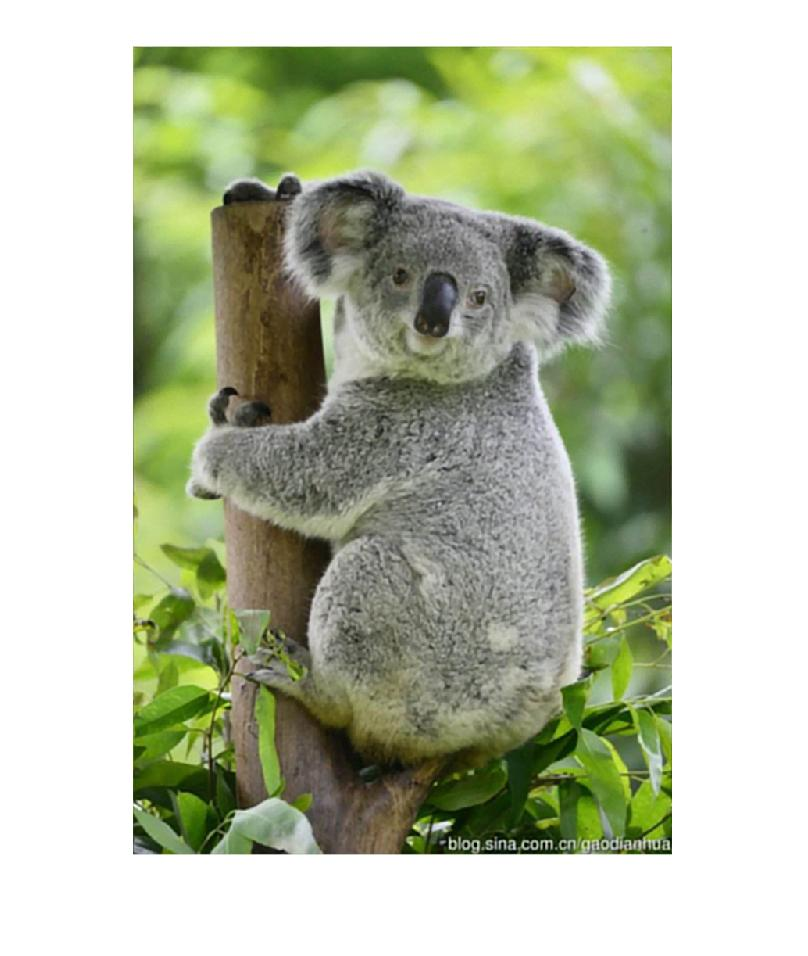
\includegraphics[width=\linewidth]{koala_recovered_cyclic.jpg}
	\end{minipage}
\end{figure}

\begin{figure}
	\caption{\textbf{Experimental Results for Non- Periodic Boundary Condition:} The picture on the left is the blurred image, on the right the recovered}
	\begin{minipage}{.5\linewidth}
		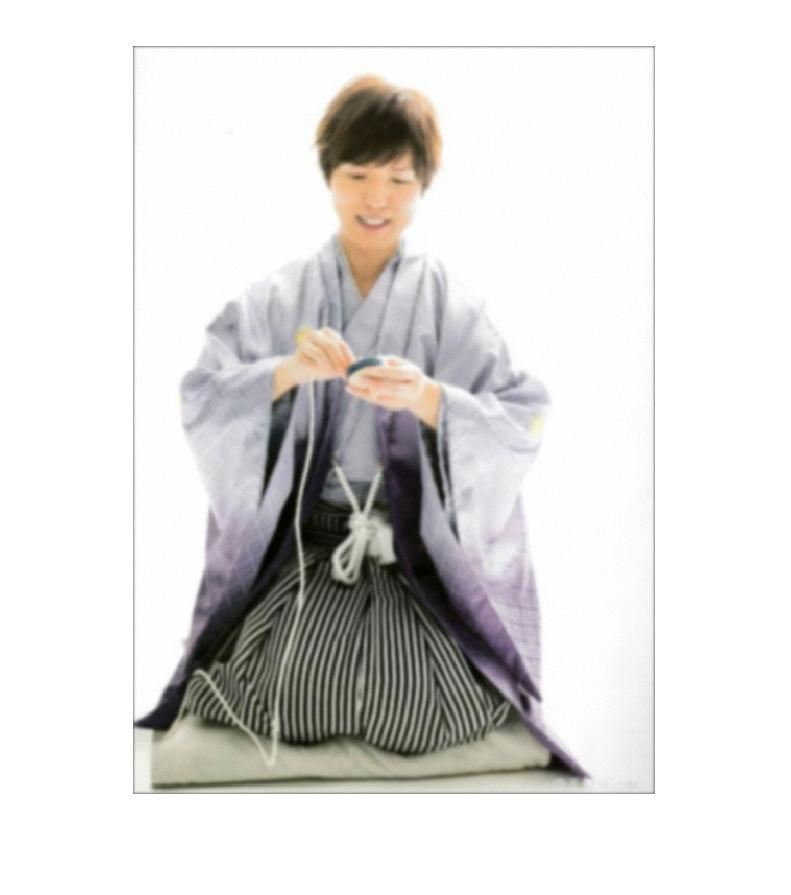
\includegraphics[width=\textwidth]{kamiya_blurred.jpg}
	\end{minipage}
	\begin{minipage}{.5\linewidth}
		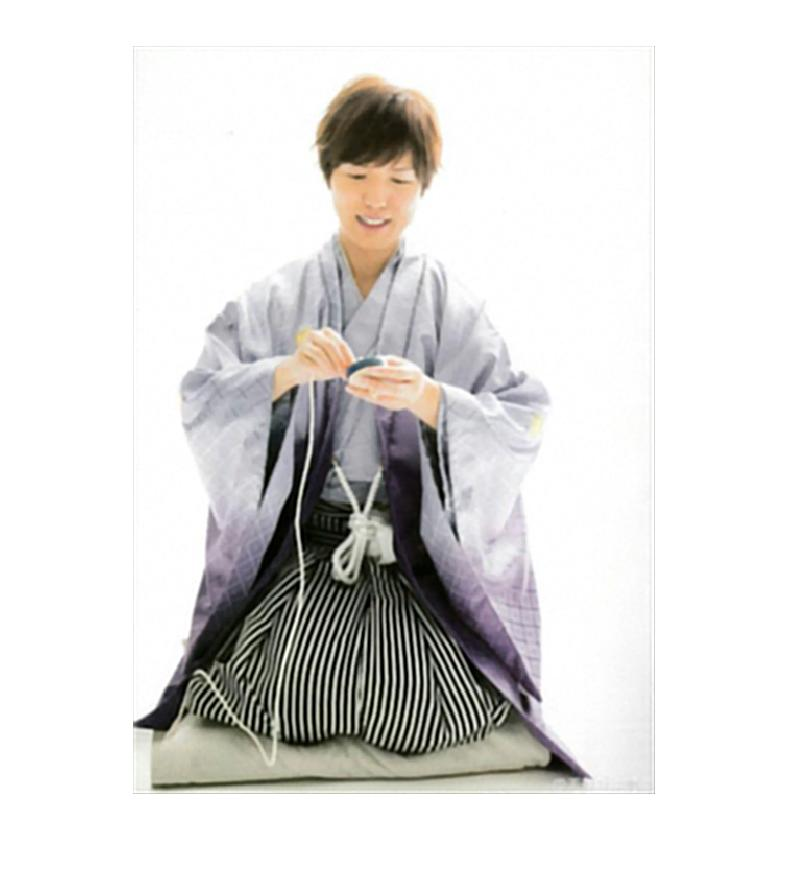
\includegraphics[width=\linewidth]{kamiya_recovered.jpg}
	\end{minipage}
	\begin{minipage}{.5\linewidth}
		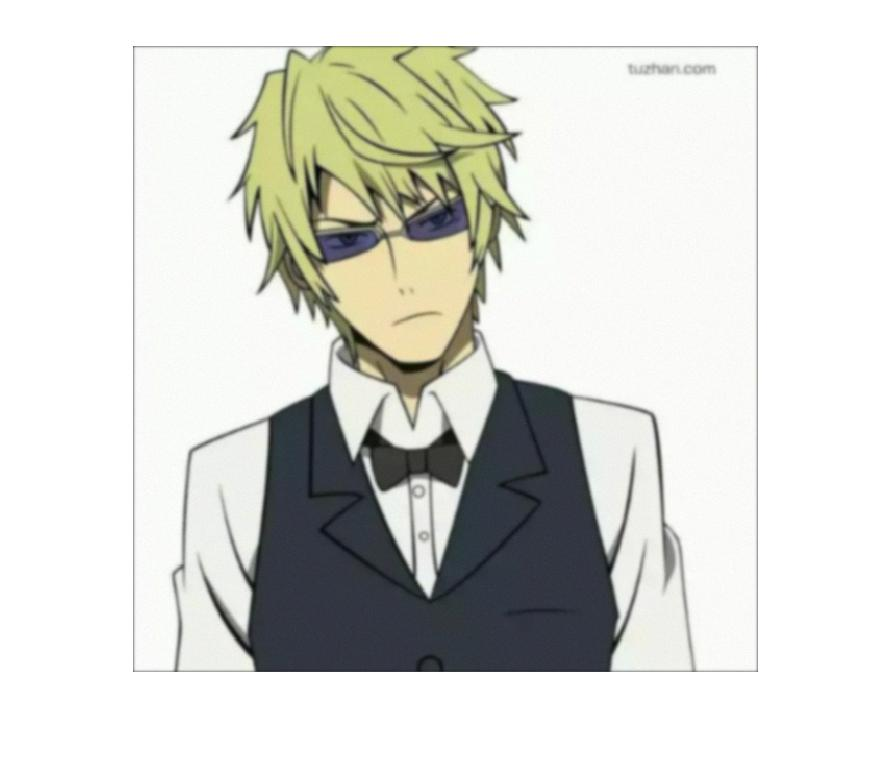
\includegraphics[width=\textwidth]{shizuwo_blurred.jpg}
	\end{minipage}
	\begin{minipage}{.5\linewidth}
		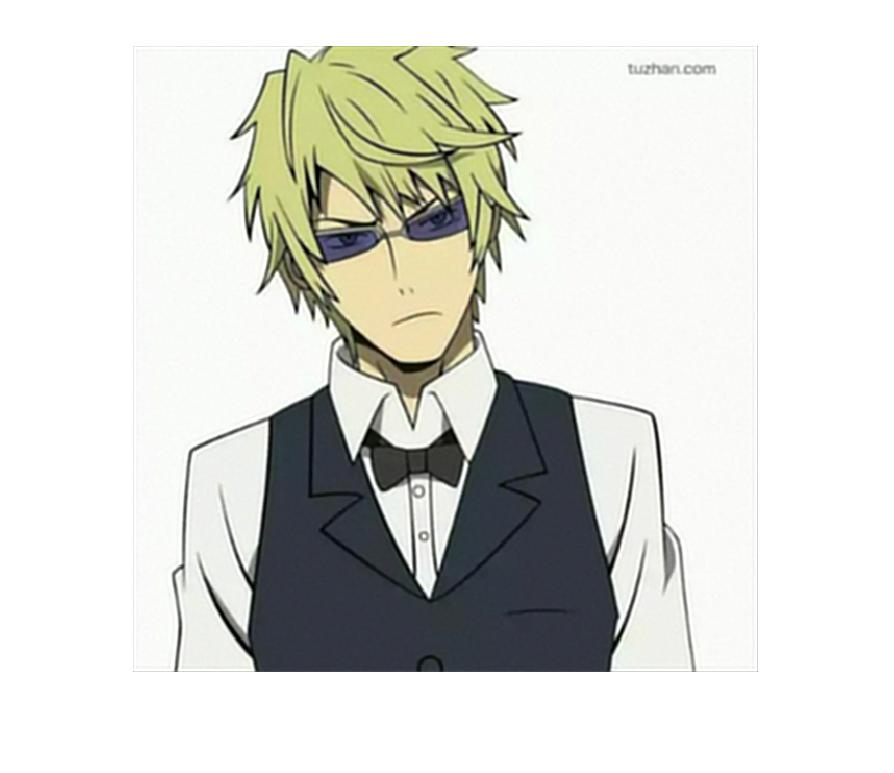
\includegraphics[width=\linewidth]{shizuwo_recovered.jpg}
	\end{minipage}
	\begin{minipage}{.5\linewidth}
		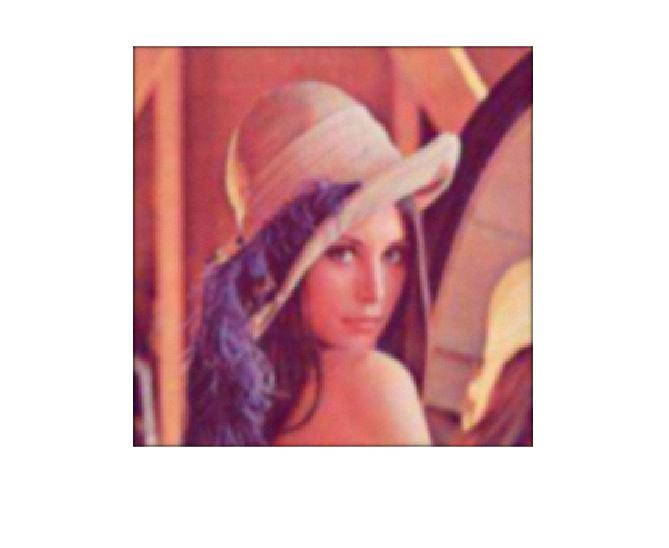
\includegraphics[width=\textwidth]{classic_blurred.jpg}
	\end{minipage}
	\begin{minipage}{.5\linewidth}
		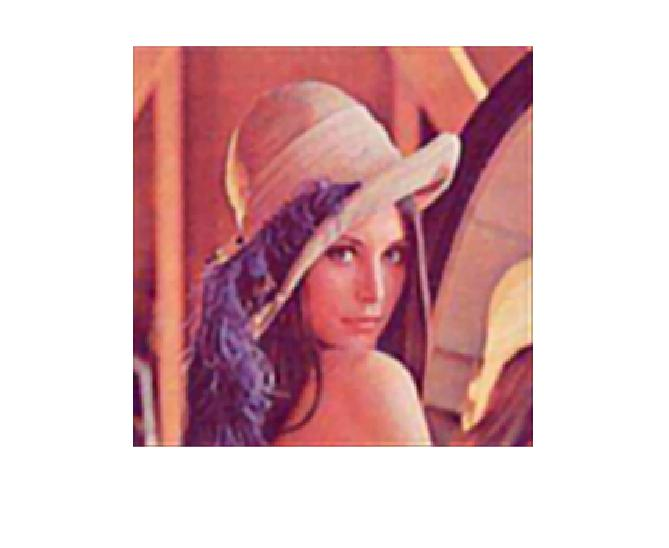
\includegraphics[width=\linewidth]{classic_recovered.jpg}
	\end{minipage}
	\begin{minipage}{.5\linewidth}
		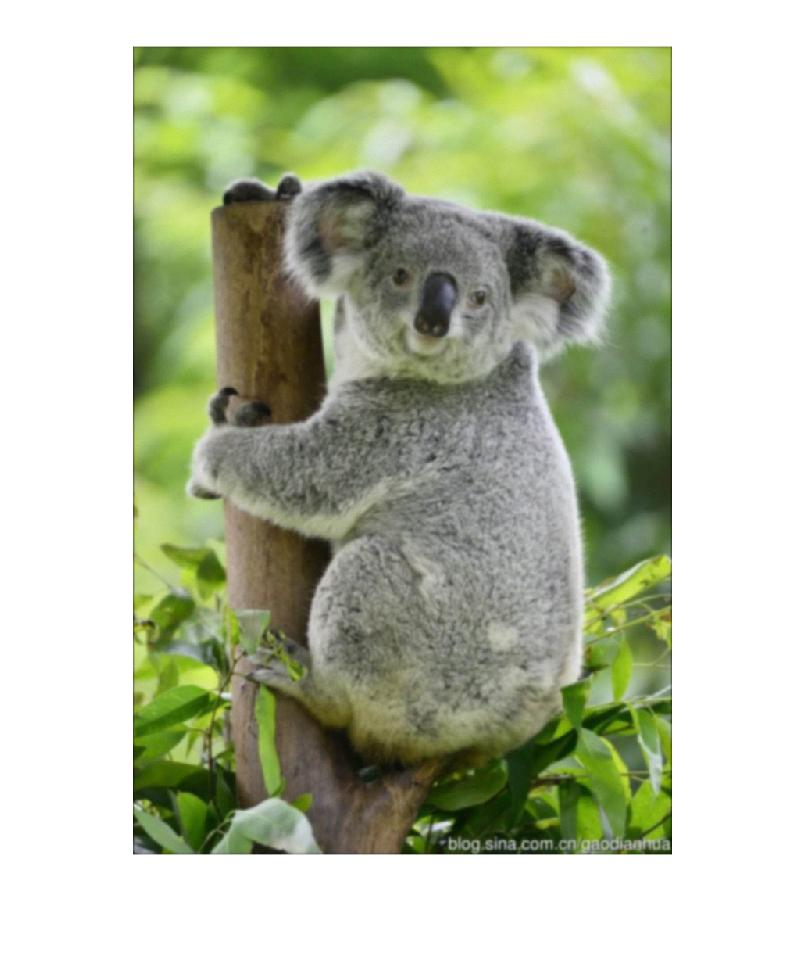
\includegraphics[width=\textwidth]{koala_blurred.jpg}
	\end{minipage}
	\begin{minipage}{.5\linewidth}
		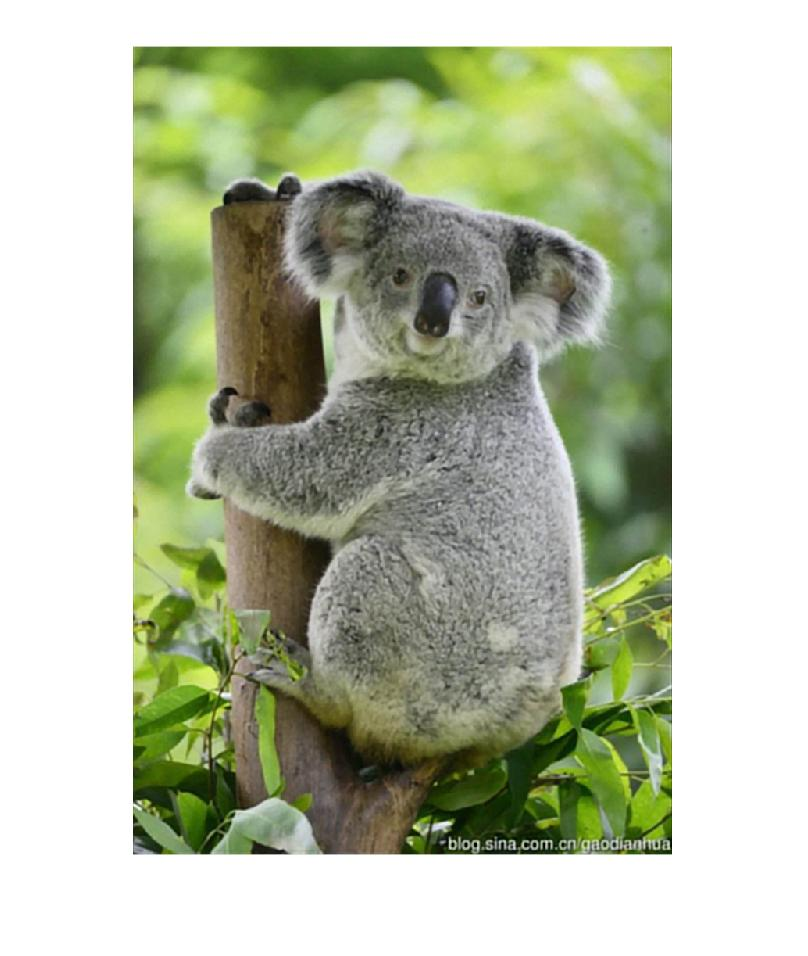
\includegraphics[width=\linewidth]{koala_recovered.jpg}
	\end{minipage}
\end{figure}
\end{document}